%https://en.bitcoin.it/wiki/Transaction
%mastering bitcoin
\Section{Transactions}\label{transactions}
Transactions in Bitcoin are not as straight forward as you might expect a transaction to be. A transaction contains a list of inputs and a list of outputs as well as some metadata like version number and lock-time. 

\begin{figure}[H]
	\centering
	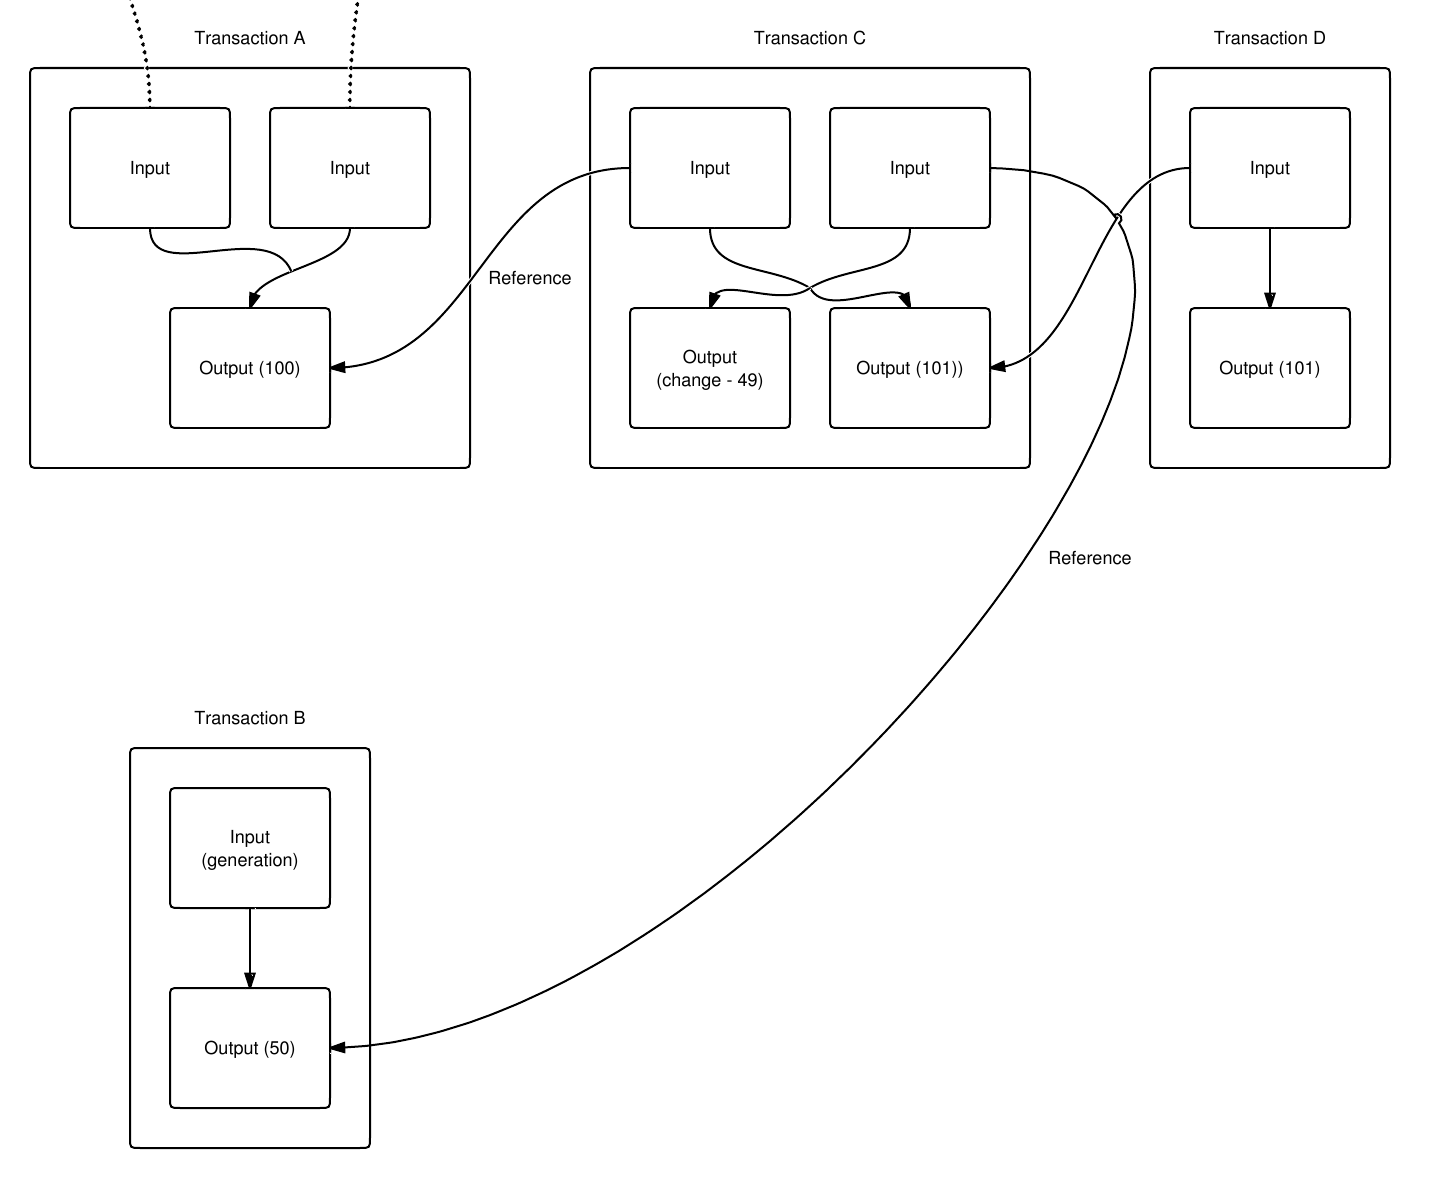
\includegraphics[width=1.0\textwidth]{background/images/transaction_basic.png}
	\caption{4 example transactions and how inputs are connected to outputs}
	\label{fig:transaction_input_output}
\end{figure}

In simplified terms an output could be seen as the destination of a transaction, in other words it says how much and to whom the transaction is sent to. An input is a reference to a previous output. The inputs take the money from the outputs they reference and that money is used to fun the new outputs. 

The inputs and outputs is where Script comes into the picture. Both outputs and inputs contains an incomplete script, together however they complete the script. The script in an output could be seen as a challenge, and the script in the input is the response. When a transaction is tested for validity the input script is appended to the script in the output and is executed. If the script comes out as valid the transaction is also valid. Here is a basic example: Let's say Alice wants to send a transaction to whoever can answer the very complex equation $4+3$. Her transaction output would contain the script:

\texttt{4 3 OP\_ADD OP\_EQUALS}

If this is executed as is it is invalid. But let's say Bob knows the answer to the equation he can then create a new transaction where the input contains the script: 

\texttt{7} 

Just as before this script is not valid by itself. But then the transaction is checked for validity the input will be appended to the start of the output script forming the following: 

\texttt{7 4 3 OP\_ADD OP\_EQUALS}

Which is a valid script, thus bobs new transaction is also valid and he may spend the money as he see fits. 

Obviously most transactions on the Bitcoin blockchain are not this simple. The most common form of transaction contians a script called P2PKH which stands for Pay to public key hash. Before we can go into details on this one however we first need to know about how signatures and sighash work in script and transactions.

\Subsection{Signatures and sighash}
Section \ref{ecdsa} covers public keys and signatures in depth.

Perhaps the most important operation in script is the \texttt{OP\_CHECKSIG} operation and its cousins. \texttt{OP\_CHECKSIG} pops two values from the stack, if the script is correctly implemented these two values should be the public key and a signature that was signed with the private key that was used to create the public key. 

The question is: what is signed when the signature is created? Broadly speaking it is the hash of the transaction that is trying to spend the output, this is not entirely correct however. Appended to the signature that is a flag called \textbf{sighash}. The value of sighash tells the script interpreter what hash was signed during the creation of the signature. There are 4 types of sighash implemented:

\Subsubsection{SIGHASH\_ALL}
This can be considered the default sighash, if it is not specified it can safely be assumed that this type was used. This simply means that the entire transaction is signed with all outputs and all other inputs.


\Subsubsection{SIGHASH\_NONE}
This one signs the transaction butwithout the outputs, it could be thought of as ''I don't care where the money goes''

\Subsubsection{SIGHASH\_SINGLE}
All outputs are removed except the output with the same index as the input that is being signed, then that transaction is signed.

\Subsubsection{SIGHASH\_ANYONECANPAY}
Signs the transaction with all the outputs but none of the other inputs. This basically means ''The money has to go here, but I don't care if someone else want to fund this transaction also''

\Subsubsection{More detailed process}
On the next page the entire signing process for SIGHASH\_ALL is detailed. This is how it is performed in the actual implementation:
\newpage
\centerline{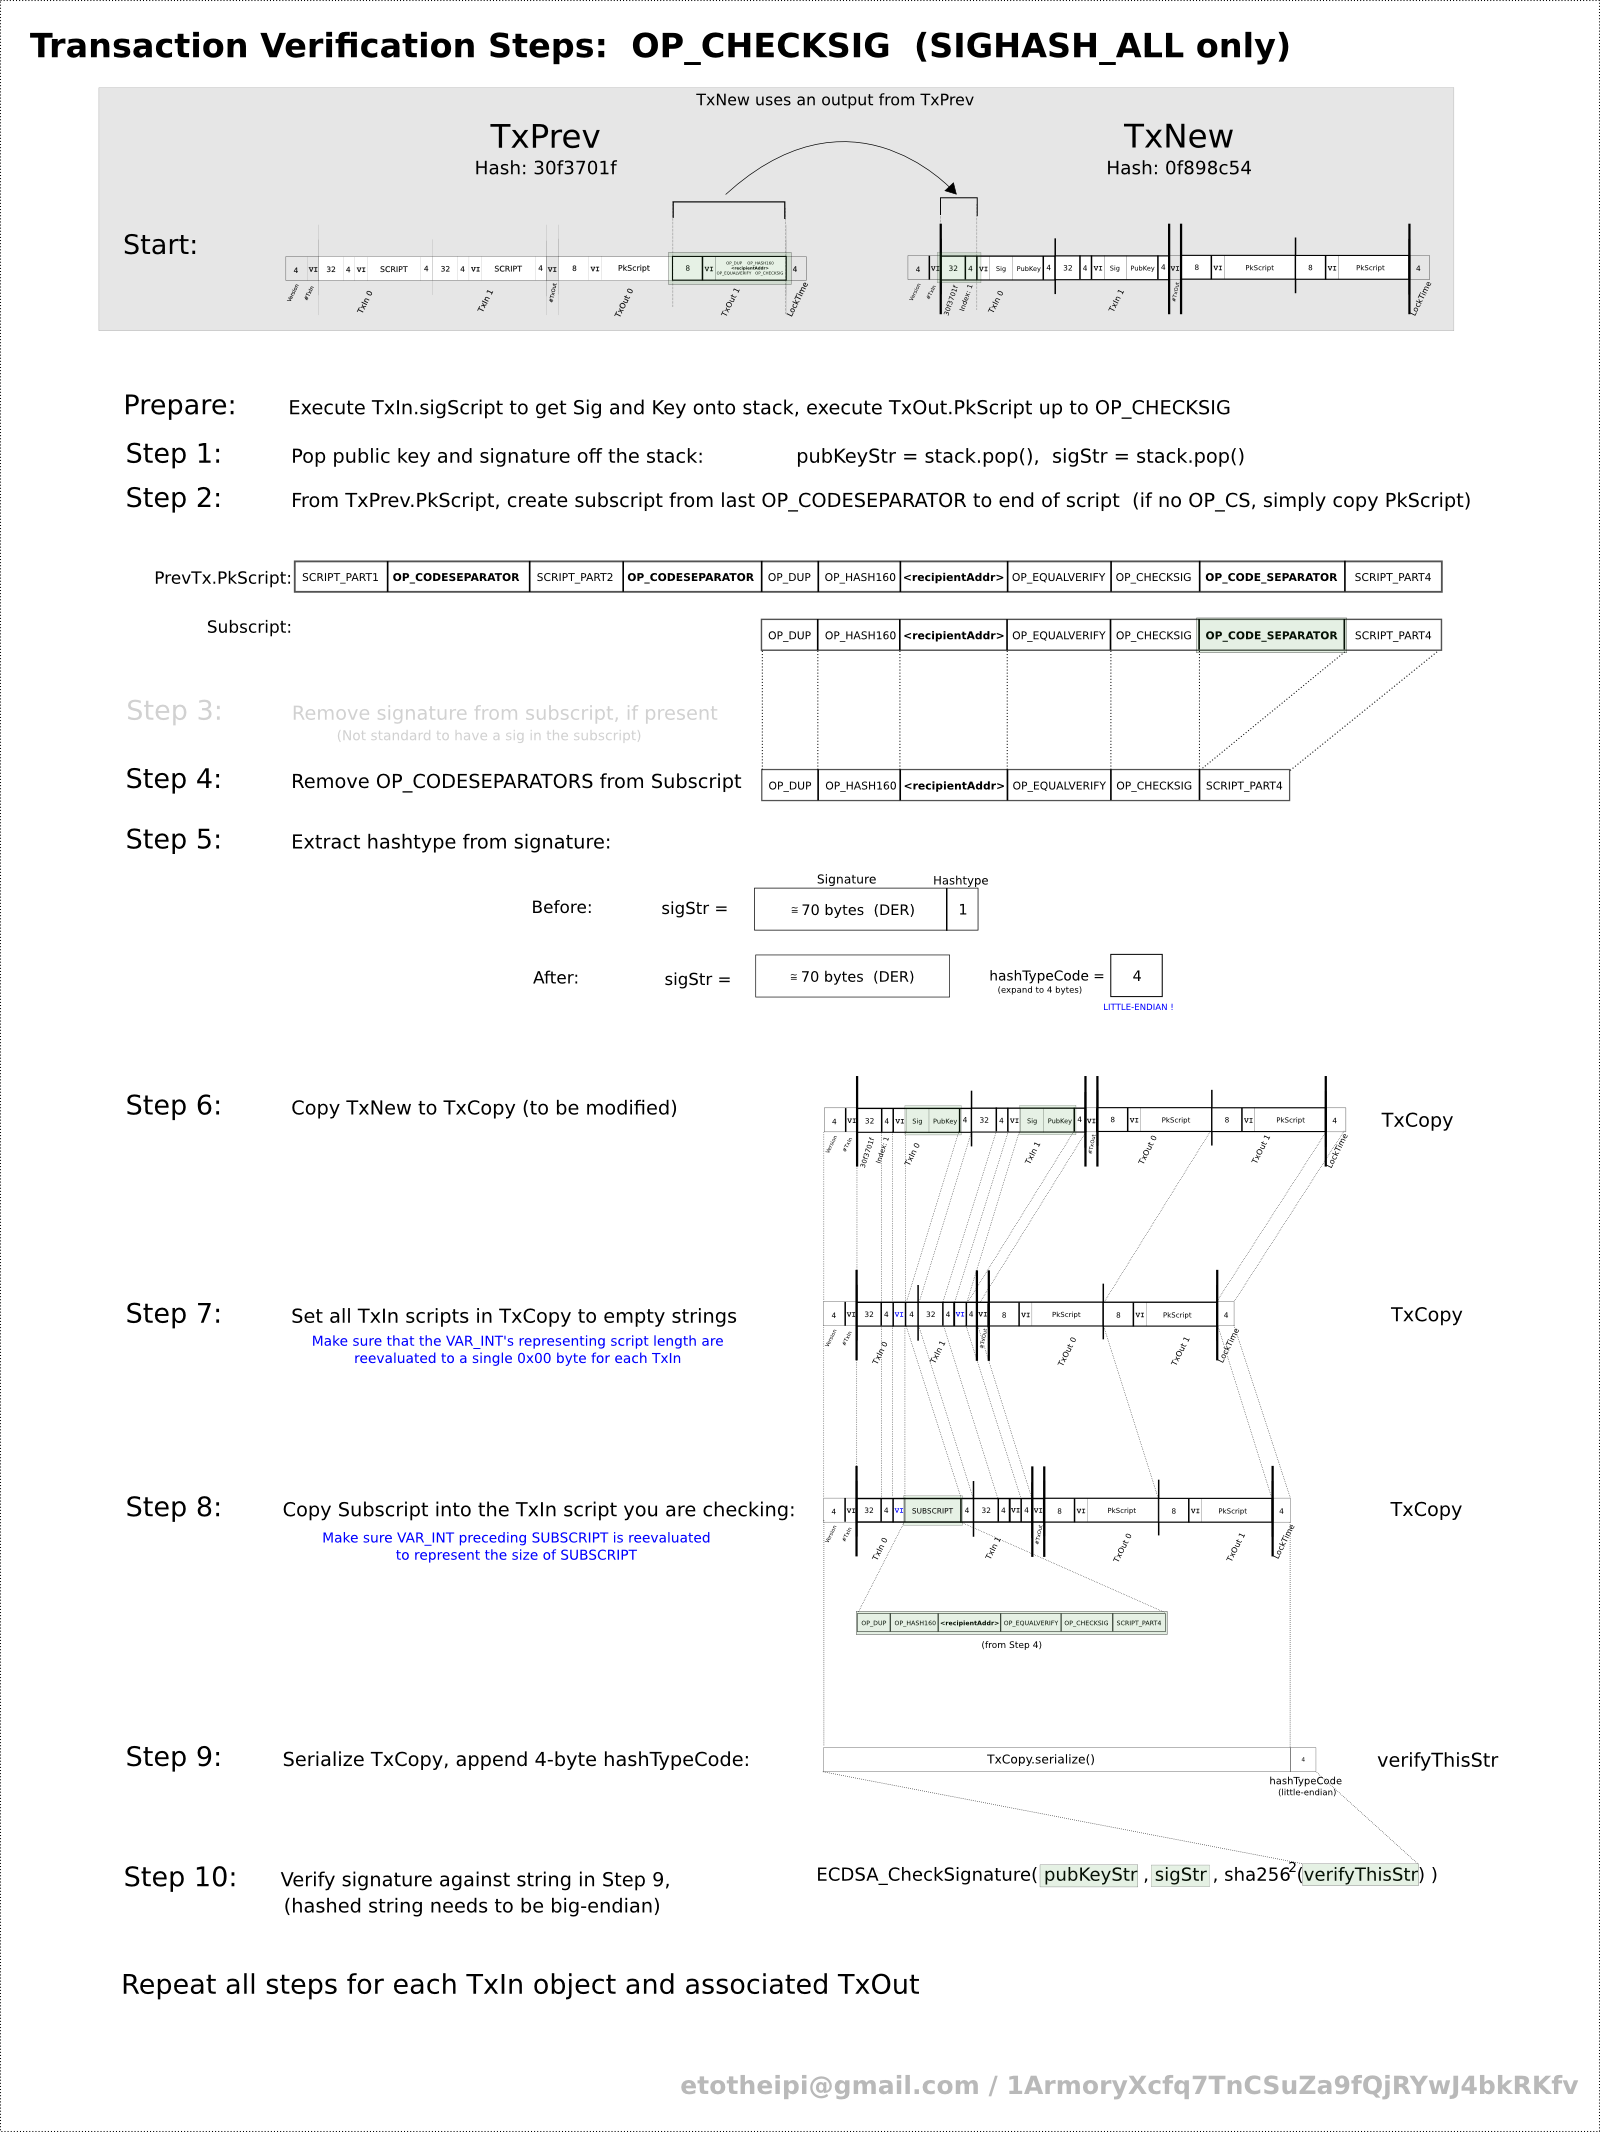
\includegraphics[width=1.35\textwidth]{background/images/checksig_in_detail.png}}
\newpage



\Subsection{Pay to public key hash (P2PKH)}
\Subsection{Pay to script hash (P2SH)}
\Subsection{Timelock and sequence}